\section{Introduction}

Binary firmware is vital in cyber-security, where understanding the purpose and functionality of compiled code is essential for reverse engineering. Traditionally, this process relies heavily on the use of decompiled binary code. This is further complicated when using microcontrollers as firmware and assembly instructions are linked to hardware peripherals, as these components are integrated and lack explicit representation in the Instruction Set Architecture (ISA) of a microprocessor.

Recent advancement in Artificial Intelligence (AI) has thrust Large Language Models (LLMs) into the foray as they are capable of interpreting and generating human-readable programming languages. This proficiency in code interpretation suggests a chance to utilize these capabilities for binary firmware analysis.






\section{Related Work}
% talk about llms for code analysis

This project was large in part inspired by the work of \cite{fang2024large} in
their use of LLMs for code analysis, where ChatGPT was used.

\section{Methodology}

\subsection{LLM Selection}

\begin{itemize}
  \item GPT-4o: GPT-4o is OpenAI's flagship chat model. We select it to measure
  how an advanced generic foundation model performs without any fine-tuning on
  our problem task.

  \item GPT-4-turbo: This model is what OpenAI provides for their fine-tuning
  service that they call "custom GPTs" wherein as users we can upload
  supplementary files (such as documentation) and provide a "system" prompt for
  the user to fine-tune the model's responses. In this case we simply gave it the system prompt shown in figure \ref{fig:system}.
\end{itemize}

\begin{figure}[!htb]
    \centering
    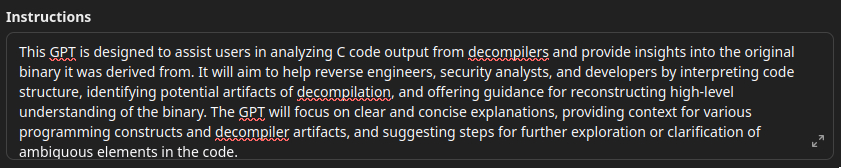
\includegraphics[width=0.9\linewidth]{2024-12-13-22-13-20-ChatGPT_Mozilla_Firefox.jpg}
    \caption{System prompt for rudimentary fine-tuning of gpt4-turbo}
    \label{fig:system}
\end{figure}

\subsection{Dataset}

For our data-set we selected two sets of C codes: one that was platform-agnostic
and one targeted for the Nordic line of Microprocessors and Peripherals. The platform agnostic code consists of the stream, whetstone benchmark, and the winner for best utility in the 27th IOCCC: an md5sum checksum utility. \cite{iocccilya} 
% some stuff on the Nordic code

Note that all codes were compiled with the same flags (excluding necessary linker flags) that being \verb|-Os -s| to both minimize token usage and eliminate information that could arise from names corresponding to certain memory addresses. 

\subsection{Experiments}

For each model given the above prompts we provide the original binary in 2 forms: a disassembled form specific to the architecture it was originally compiled on (x86 for the agnostic code and arm32 for the nordic code), and a raw de-compiled from taken from the analysis of the ghidra de-compiler. 

\subsubsection{Prompt Construction}

Aside from the special system prompts for each of the models, each was provided 3 prompts in the form of: "\{code\} Analyze this \{code variant\} and tell me its function and purpose?", "What sort of inputs does the de-compiled code take?", "What sort of output does the code emit?".

\section{Results}
\subsection{Stream Benchmark}

The stream benchmark we selected as basic and easily interpretable example as a sanity check of the both model's initial performance. With the amount of explicit strings in both the decompiled and the disassembled code both models were able to easily surmise the nature of the benchmark: that being to measure system memory bandwidth. When asked about the type of input the code takes only the system prompted turbo model was unable to deduce that the benchmark is self contained taking no input. When asked about the output the decompiled case for both models were able to emit a nearly perfect output that the benchmark would've gotten had it been executed. However, in the disassembled case the 4o model was only able to deduce the numerical outputs and not the prefix output that is always emitted from running the benchmark.

\subsection{Whetstone Benchmark}

Our selection of the Whetstone benchmark next was to select a code that provided less string information for either model to glean information from. Despite such a decision in both the disassembled and decompiled cases both the fine-tuned model and the generic model are able to both interpret that the whetstone benchmark is a numerical performance benchmark. GPT4o on top of surmising this though not explicitly saying so makes note that "a key feature of benchmarks like Whetstone or LINPACK." with the codes' usage of \verb|time@plt|. This time only the GPT4o was able to accurately predict the output of the code. From which we can possibly surmise that both models are primarily matching against the type of system calls to interpret the nature of this code. 

\subsection{2020 IOCCC - Best Utility}

For an obfuscated codes we selected the 2020 winner for best utility by Ilya
Kurdyukov: an md5sum checksum utility. \cite{iocccilya} When queried on what could be the purpose of the code surprisingly the case that performed the worst was the gpt4o model with the decompiled code concluding that the was some code that was cryptography or puzzle related whereas the other 3 cases were able to surmise that the code was some hashing algorithm and surmised it to be the md5sum algorithm. Like the previous examples, when queried on the inputs and outputs of the code the same continued as when asked about the purpose where the gpt4o model on the decompiled code was only able to reason that the algorithm took text input and output some form of output. Otherwise from the output there seems to be no indication that it understood what the code did. The difference in performance with the turbo model and the 4o model we surmise could be with how the 4o model is tokenizing the output in the disassembled case both model's were able to accurately conclude the purpose and algorithm.

\begin{figure}[!htb]
    \centering
    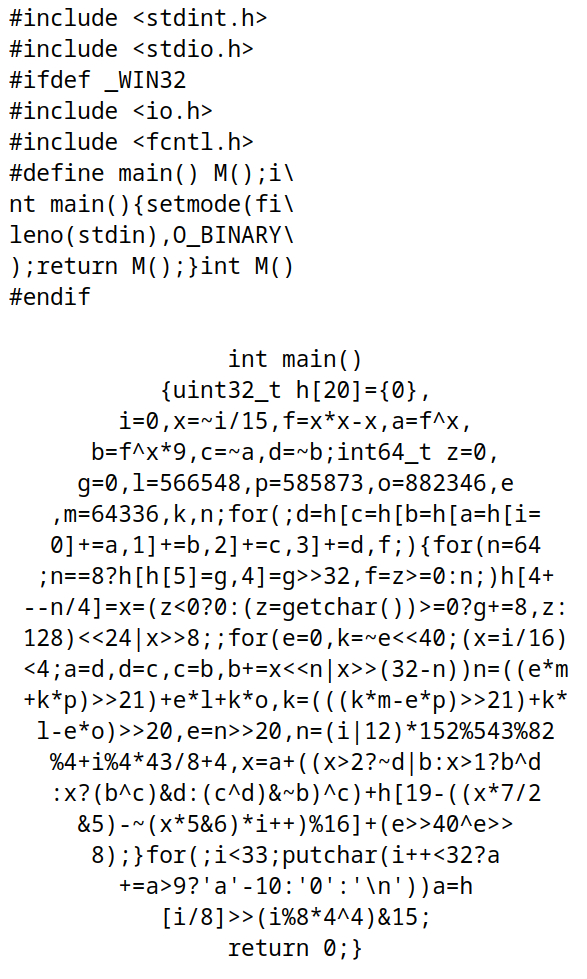
\includegraphics[width=0.5\linewidth]{2024-12-13-22-45-32-ioccc_org_2020_kurdyukov1_prog_c_qutebrowser.jpg}
    \caption{obfuscate example from IOCCC \cite{iocccilya}}
    \label{fig:enter-label}
\end{figure}

\subsection{nrf gpio tasks and events}

For this code we took one of the example codes provided in the nRF5 17.1 SDK for GPIO read and write tasks. In particular the code instantiates a timer and the states of GPIO pins and periodically writes to those set pins to blink an led connected to the micro-controller. Other than the architecture being different the binaries themselves were compiled as flat binaries with much of the avaliable function calls signatures removed as was common in the previous codes which were elf binaries targeting linux with an explicit calling convention and set of signatures. With all cases the model's were unable to surmise what the code was doing and in the initial query all the models conclude that the code could possibly be either a fuzzer or some form of malicious binary. When asked on the nature of the inputs and outputs only the disassembled turbo model was able to hint towards the code possibly being related to hardware driven outputs while the other cases the names generated by the decompilers often confused the models leading them to talking about the nature of specific lines of the code rather than what blocks did wholistically. 

\subsection{Discussion}

From these codes we find that much of the information the large language models glean and use to interpret are based off the humanreadable signatures emitted particularly when compiled for a generic operating system: requiring consistent abi comparability between applications. Even in the md5sum case we note that the code itself has "magic" numbers as one would call it that are distinct signatures of the md5sum algorithm. These assumptions fall apart when either model is given the binary analysis output of a flat self-contained binary targetting embedded arm code as we found the names generated from the decompiler often confused and made the models focus on specific lines rather than the purpose of whole sections of code. 

\section{Future Work}

Our method had three key limitations: Not properly fine-tuning on a large number of examples and, not having jump locations in the disassembled cases, and with larger binaries and function definitions and not
having explicit representations of the control flow graph of the provided
binary that could be emitted from a tool such as \verb|angr|. Similar to how Wang et. al. \cite{wang2024llamameshunifying3dmesh} tokenize their mesh, data we could do similar on both the control flow graph denoting a node-edge format where nodes can be enumerated and edges in the form of (e \{source node\} \{\verb|br|/\verb|jmp| true\} \{\verb|br|/\verb|jmp| false\}) and each node is a block of unbranched assembly as shown in Figure \ref{fig:cfg}. With such a representation, we could represent each unbranched assembly block as a vector in a RAG database which could prove particularly useful for larger binaries that surpass the context window length.



\begin{figure}
    \centering
    \includegraphics[width=0.9\linewidth]{2024-12-12-21-21-54-Cutter_–_a_out.jpg}
    \caption{preview of control flow graph for obfuscated md5sum code \cite{iocccilya}}
    \label{fig:cfg}
\end{figure}

% talk about llama mesh

\section{Conclusion}

We extended the work of Fang et al. \cite{fang2024large} into the realm of decompiled code analysis. Our findings reveal that current language models, while capable of basic code analysis, largely depend on the human-readability of the code and its similarity to publicly available, "in-the-wild" examples to draw conclusions. When faced with flattened or overly convoluted naming conventions, as often produced by decompilers, these models can underperform compared to their performance on disassembled code, frequently failing due to the repetitive and abstract nature of the tokens. This highlights a key limitation: models primarily trained on human-readable outputs struggle to analyze highly specialized or hardware-specific code effectively. Future research should address these challenges, even if it means that models, with sufficient training data, may function more as repositories for algorithmic signatures rather than employing the nuanced reasoning humans use to interpret code.
